\documentclass[12pt]{article}
\usepackage[margin=1in]{geometry}
\usepackage{amsmath, amsthm, amssymb, amsfonts, pbox, graphicx}
\usepackage[colorlinks = true, linkcolor = black, urlcolor = blue]{hyperref}

\makeatletter
\renewcommand*{\eqref}[1]{%
  \hyperref[{#1}]{\textup{\tagform@{\ref*{#1}}}}%
}
\makeatother

\newtheorem{theorem}{Theorem}
\theoremstyle{definition}
\newtheorem{problem}{Problem}
\renewcommand*{\proofname}{Solution}
\newenvironment{custompbm}[1]
  {\renewcommand\theproblem{#1}\problem}
  {\endproblem}
\renewcommand{\theenumi}{\alph{enumi}}

\newcommand{\E}{\text{E}}
\newcommand{\V}{\text{Var}}
\newcommand{\Co}[2]{\text{Cov}\left({#1}, {#2}\right)}
\newcommand{\pdf}{\text{pdf}}
\newcommand{\pmf}{\text{pmf}}
\newcommand{\me}{\mathrm{e}}
\newcommand*\diff{\mathop{}\!\mathrm{d}}
\newcommand{\vect}[1]{\boldsymbol{#1}}
\newcommand{\mx}[1][t]{\mu_X({#1})}
\newcommand{\gx}[2]{\gamma_X({#1}, {#2})}
\newcommand\norm[1]{\left\lVert#1\right\rVert}

\graphicspath{ {images/} }

\title{MATH 635 Final Assessment}
\author{Matthew Tiger}


\begin{document}


\maketitle


\begin{problem}{1}
  Suppose that the number of claims each policy holder will have in a given year is
  Poisson distributed with mean randomly distributed with density function $g(\lambda) = e^{-\lambda}$
  for $\lambda \geq 0$.
  What is the probability that a policy holder will have $n$ claims in that year?
\end{problem}

\begin{proof}
  Let $X$ be the discrete random variable representing the number of claims
  a policy holder will have in a given year. Let $Y$ be the continuous random
  variable representing the Poisson parameter $\lambda$ with density function
  $g(\lambda) = e^{-\lambda}$ with $\lambda \geq 0$.

  Conditioning the probability that $X = n$ on the random variable $Y$ shows
  that
  \begin{align*}
    P(X = n) &= \int_{-\infty}^{\infty} P(X=n | Y=\lambda) g(\lambda) d \lambda \\
    &= \int_{0}^{\infty} P(X=n | Y=\lambda) e^{-\lambda} d \lambda
  \end{align*}
  where the limits of integration have changed since $P(X=n | Y=\lambda) = 0$ for
  $\lambda < 0$ given our initial assumptions. Using the probability mass function
  for the Poisson random variable $X$ in conjunction with the fact that for
  $Y=\lambda$ the random variable $X$ will have parameter $\lambda$,
  we see that
  \begin{align*}
    P(X=n | Y=\lambda) = \frac{e^{-\lambda}\lambda^n}{n!}.
  \end{align*}
  Thus, from the above computation, we have that
  \begin{align*}
    P(X = n) &= \int_{0}^{\infty}  e^{-\lambda} \left[\frac{e^{-\lambda}\lambda^n}{n!}\right] d \lambda \\
    &= \frac{1}{n!}\int_{0}^{\infty} \lambda^n e^{-2\lambda} d\lambda.
  \end{align*}
  Making the $u$-substitution $u=2\lambda$, the previous integral transforms into
  \begin{align*}
    P(X = n) &= \frac{1}{n!}\int_{0}^{\infty} 2^{-(n+1)}u^{n} e^{-u} du \\
    &= \frac{2^{-(n+1)}}{n!}\int_{0}^{\infty} u^{n} e^{-u} du \\
    &= \frac{2^{-(n+1)}\Gamma(n+1)}{n!} \\
    &= 2^{-(n+1)},
 \end{align*}
 where we have used the fact that, for an integer $k$,
 \begin{align*}
   \Gamma(k) = \int_0^\infty x^{k-1} e^{-x} dx = (k-1)!.
 \end{align*}

 Therefore, the probability a policy holder will have $n$ claims in that year is $2^{-(n+1)}$.
\end{proof}
\newpage


\begin{problem}
  Consider the differential equation
  \begin{align}\label{diffeq}
    y'' - y = -x,\quad  0<x<1 \quad y(0) = y(1) = 0
  \end{align}
  as in Example 15.12 on page 502.
  Use the basis $\{\phi_j(x)\} = \{x^j(1-x)^j\}$, as in section 15.5.1, to
  compute approximations to the exact solution using the finite-element method.

  Provide relative errors at the points 0.25, 0.50, and 0.75 of the approximations
  using the first $n=2,3,4$ basis functions. Plot
  the corresponding approximations $y_2$, $y_3$, $y_4$, and the exact solution
  $y$. Then find the first value of $j$ for which the relative error at all
  three points is less than 0.5\%.
\end{problem}

\begin{proof}
  The differential equation presented in the problem is a second order linear
  differential equation. It is easily shown that the homogeneous solution is
  given by $y_h(x) = c_1 e^{-x} + c_2e^{x}$ and that a particular solution is
  given by $y_p(x) = x$. Thus the general solution is $y(x) = c_1 e^{-x} + c_2e^{x} + x$.
  Using the boundary conditions, we see that the exact solution is
  \begin{align}\label{exact}
    y(x) = \frac{e^{x}e}{1-e^2} -\frac{e^{-x}e}{1-e^2} + x
  \end{align}

  We now wish to approximate the exact solution $y(x)$.
  Note that the exact solution to the differential equation \eqref{diffeq} is
  a continuous function. This fact combined with the fact that $\{\phi_j(x)\}$
  form a basis of the function space shows that the continuous function $y(x)$
  can be approximated with a linear combination of the basis functions.
  Therefore, we wish to find an approximation $y_n(x)$ to the exact solution
  $y(x)$ where
  \begin{align}\label{finite_approximation}
    y_n(x) = \sum_{j=1}^n a_j \phi_j(x).
  \end{align}
  Note that our basis functions $\{\phi_j(x)\}$ satisfy the boundary
  conditions, i.e.\ $\phi_j(0) = \phi_j(1) = 0$ so that $y_n(x)$ also satisfies the
  boundary conditions.

  Corollary 15.2 suggests that if
  \[
    \int_0^1 (y_n'' - y_n + x)\phi_i(x) dx = 0 \quad \text{for $i=1,\dots,n$}
  \]
  then $y_n'' - y_n + x = 0$, i.e\ $y_n(x)$ satisfies the differential
  equation \eqref{diffeq}. If $y_n(x)$ satisfies the
  differential equation and the boundary conditions, then we know that $y_n(x)$
  approximates the exact solution $y(x)$.

  Therefore, we choose the coefficients $a_j$ such that they satisfy the system of
  equations
  \begin{align}\label{first_system}
    \sum_{j=1}^n a_j \int_0^1 \phi_j''(x)\phi_i(x) - \phi_j(x)\phi_i(x) dx = -\int_0^1 x \phi_i(x) dx \quad \text{for $i=1,\dots,n$}.
  \end{align}

  The above system unnecessarily uses the second derivative of the basis
  functions. We can rewrite the coefficients of the above system to use only
  the first derivative of the basis functions. To see this,
  note that we can rewrite the differential equation \eqref{diffeq} in the form
  \begin{align}\label{alternate_diffeq}
    (p(x)y')' + q(x)y' + r(x)y = f(x)
  \end{align}
  by choosing $p(x) = 1$, $q(x) = 0$, $r(x) = -1$, and $f(x) = -x$. With this form of the
  differential equation we would require the approximation \eqref{finite_approximation}
  to satisfy the following equations
  \[
    \int_0^1 ((p(x)y_n')' + r(x)y_n)\phi_i(x) dx = \int_0^1f(x)\phi_i(x)dx \quad \text{for $i=1,\dots,n$}.
  \]
  Making use of the fact that the basis functions are 0 on the boundary we see that
  \begin{align*}
    \int_0^1(p(x)y_n')'\phi_i(x) dx
    &= \phi_i(x)p(x)y_n'\rvert_0^1 - \int_0^1 p(x)y_n'\phi_i'(x) dx \\
    &= - \int_0^1 p(x)y_n'\phi_i'(x) dx.
  \end{align*}
  With this and the definitions of the functions $p(x)$, $r(x)$, and $f(x)$,
  the system of equations \eqref{first_system} becomes
  \begin{align}\label{system_imp}
    \sum_{j=1}^n a_j \int_0^1 -\phi_j'(x)\phi_i'(x) - \phi_j(x)\phi_i(x) dx = -\int_0^1 x \phi_i(x) dx \quad \text{for $i=1,\dots,n$}.
  \end{align}

  Finding the solution to the system of equations \eqref{system_imp} identifies
  the coefficients $a_j$ that define our approximation.

  In this instance, we have chosen the basis $\left.\{\phi_j(x)\}\right._{j=1}^n$ where $\phi_j(x) = x^j(1-x)^j$.
  Thus,
  \begin{align*}
    \phi_j'(x)
    &= \left(x^j\right)'(1-x)^j + x^j\left((1-x)^j\right)' \\
    &= jx^{j-1}(1-x)^j -jx^j(1-x)^{j-1}
  \end{align*}
  for $j=1,\dots,n$.
\end{proof}

\begin{problem}
  Repeat problem 2 with the basis $\{ \sin(j\pi x)\}$.
\end{problem}

\begin{proof}
  We use the same methods outlined in the solution to problem 2 to obtain an
  approximation using the basis $\{\phi_j(x) \}$ with $\phi_j(x) = \sin(j\pi x)$.
  Now we see see that,
  \begin{align*}
    \phi_j'(x)
    &= j\pi \cos(j\pi x)
  \end{align*}
  for $j=1,\dots,n$.

  Using the MATLAB function $\texttt{approximation.m}$, we construct the above
  system of equations and solve them arriving at approximations to the exact
  solution for $n=2,3,4$.
  The tables comparing the exact solution to these approximations at the
  points $x=0.25, 0.50, 0.75$ can be found below.

  \begin{table}[h!]
    \centering
    \bgroup
    \def\arraystretch{1.75}
    \begin{tabular}{| l | c | c | c | c |}
      \hline
      $x$ & $y(x)$ & $y_{2}(x)$ & $|y(x) - y_{2}(x)|$ & \pbox{5cm}{$\frac{100|y(x) - y_{2}(x)|}{|y(x)|}$} \\
      \hline
      0.25 & 3.504760e-02 & 3.355071e-02 & 1.496893e-03 & 4.271028 \\
      0.50 & 5.659056e-02 & 5.856881e-02 & 1.978250e-03 & 3.495724 \\
      0.75 & 5.027579e-02 & 4.927810e-02 & 9.976905e-04 & 1.984435 \\
      \hline
    \end{tabular}
    \egroup
    \caption{Comparison of approximation $y_{2}$ to solution $y$ using basis $\phi_j = \sin(j\pi x)$. All computations are rounded to 6 significant digits.}
  \end{table}

  \begin{table}[h!]
    \centering
    \bgroup
    \def\arraystretch{1.75}
    \begin{tabular}{| l | c | c | c | c |}
      \hline
      $x$ & $y(x)$ & $y_{3}(x)$ & $|y(x) - y_{3}(x)|$ & \pbox{5cm}{$\frac{100|y(x) - y_{3}(x)|}{|y(x)|}$} \\
      \hline
      0.25 & 3.504760e-02 & 3.522118e-02 & 1.735810e-04 & 0.495272 \\
      0.50 & 5.659056e-02 & 5.620640e-02 & 3.841569e-04 & 0.678836 \\
      0.75 & 5.027579e-02 & 5.094857e-02 & 6.727834e-04 & 1.338186 \\
      \hline
    \end{tabular}
    \egroup
    \caption{Comparison of approximation $y_{3}$ to solution $y$ using basis $\phi_j = \sin(j\pi x)$. All computations are rounded to 6 significant digits.}
  \end{table}

  \begin{table}[!h]
    \centering
    \bgroup
    \def\arraystretch{1.75}
    \begin{tabular}{| l | c | c | c | c |}
      \hline
      $x$ & $y(x)$ & $y_{4}(x)$ & $|y(x) - y_{4}(x)|$ & \pbox{5cm}{$\frac{100|y(x) - y_{4}(x)|}{|y(x)|}$} \\
      \hline
      0.25 & 3.504760e-02 & 3.522118e-02 & 1.735810e-04 & 0.495272 \\
      0.50 & 5.659056e-02 & 5.620640e-02 & 3.841569e-04 & 0.678836 \\
      0.75 & 5.027579e-02 & 5.094857e-02 & 6.727834e-04 & 1.338186 \\
      \hline
    \end{tabular}
    \egroup
    \caption{Comparison of approximation $y_{4}$ to solution $y$ using basis $\phi_j = \sin(j\pi x)$. All computations are rounded to 6 significant digits.}
  \end{table}


  We also provide the graphs of these comparisons in Figure \ref{trig_plot}.

  \begin{figure}[h!]
    \begin{center}
      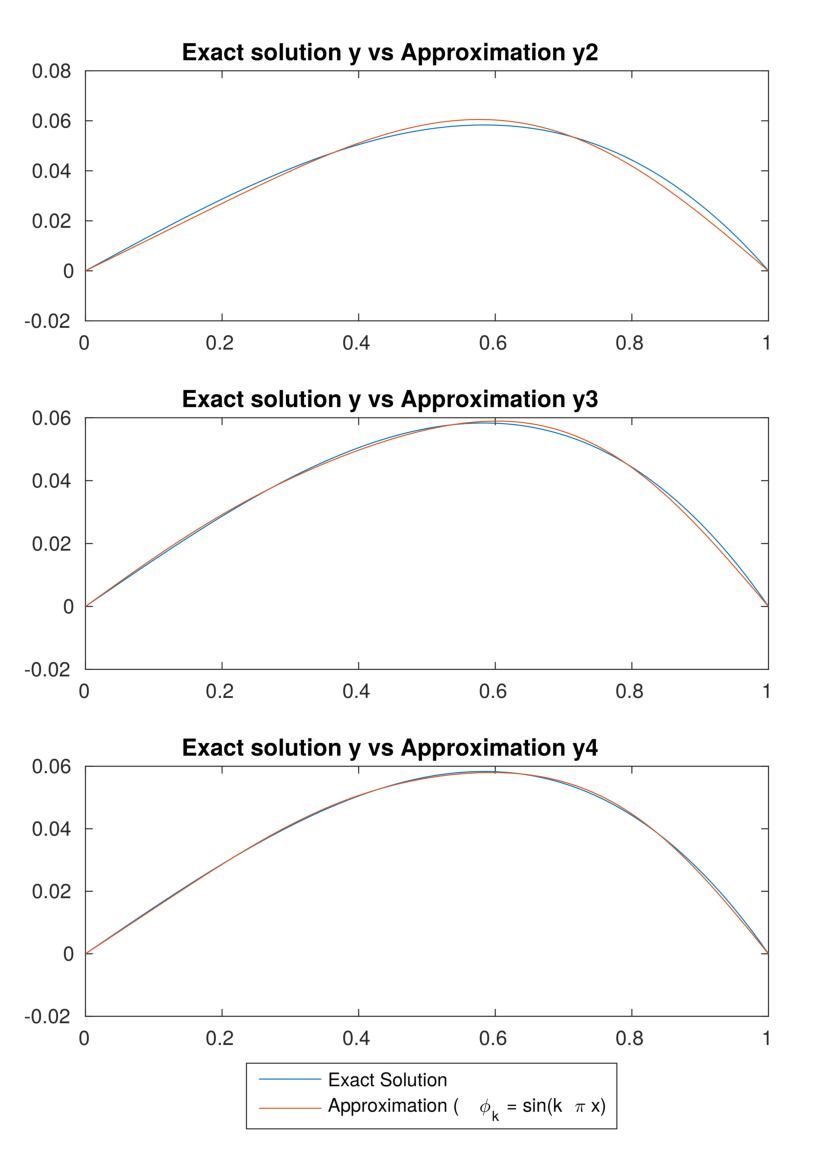
\includegraphics[scale=1.0]{trigonometric_basis_comparison}
    \end{center}
    \caption{Plots of exact solution $y$ and approximation $y_n$ over the interval $[0, 1]$
      using basis $\phi_j = \sin(j\pi x)$.}\label{trig_plot}
  \end{figure}

  The first value of $n$ such that the relative error of the approximation at
  each of the points $x_0=0.25, x_1=0.50, x_2=0.75$ is less than 5.0e-01\% is given by $n=6$.
  The relative errors $r_{x_i}$ at the above points for the approximation $y_6$ are
  $r_{x_0}$ = 3.080284e-01\%, $r_{x_1}$ = 2.293399e-01\%, and $r_{x_2}=$ 2.304205e-02\%.
  This value of $n$ needed for the relative error percents to be less than 5.0e-01\% is quite low.

  The general method of computing the coefficients suits our needs well enough
  if the goal is to obtain an approximation with a relative error less than 5.0e-01\% at these points.
  It will be mentioned, however, that the entries $a_{ij}$ of the coefficient matrix
  found in \eqref{system_imp} admit a special structure due to the choice of basis.
  Namely,
  \begin{align*}
    a_{ij} =
    \begin{cases}
      0 & \text{if $i \neq j$} \\
      \frac{-j^2\pi^2}{2} - \frac{1}{2} & \text{if $i = j$} \\
    \end{cases}
  \end{align*}

  This suggests that the coefficient matrix is actually a diagonal matrix. Finding
  the solution to the system \eqref{system_imp} is therefore trivial and reduces
  the computational complexity of finding the approximation immensely as we only need
  to compute the entries of the coefficient matrix along the diagonal and the entries
  of the column vector in the system. Additionally, a similar calculation shows
  that the integral is not needed for the column vector either as $b_i = (-1)^i / (i\pi)$.

  In order to accommodate this special structure we have created conditional creations
  of the coefficient matrices and column vectors in the code mentioned earlier.
\end{proof}



\end{document}
